\documentclass[twoside]{book}

% Packages required by doxygen
\usepackage{fixltx2e}
\usepackage{calc}
\usepackage{doxygen}
\usepackage[export]{adjustbox} % also loads graphicx
\usepackage{graphicx}
\usepackage[utf8]{inputenc}
\usepackage{makeidx}
\usepackage{multicol}
\usepackage{multirow}
\PassOptionsToPackage{warn}{textcomp}
\usepackage{textcomp}
\usepackage[nointegrals]{wasysym}
\usepackage[table]{xcolor}

% Font selection
\usepackage[T1]{fontenc}
\usepackage[scaled=.90]{helvet}
\usepackage{courier}
\usepackage{amssymb}
\usepackage{sectsty}
\renewcommand{\familydefault}{\sfdefault}
\allsectionsfont{%
  \fontseries{bc}\selectfont%
  \color{darkgray}%
}
\renewcommand{\DoxyLabelFont}{%
  \fontseries{bc}\selectfont%
  \color{darkgray}%
}
\newcommand{\+}{\discretionary{\mbox{\scriptsize$\hookleftarrow$}}{}{}}

% Page & text layout
\usepackage{geometry}
\geometry{%
  a4paper,%
  top=2.5cm,%
  bottom=2.5cm,%
  left=2.5cm,%
  right=2.5cm%
}
\tolerance=750
\hfuzz=15pt
\hbadness=750
\setlength{\emergencystretch}{15pt}
\setlength{\parindent}{0cm}
\setlength{\parskip}{3ex plus 2ex minus 2ex}
\makeatletter
\renewcommand{\paragraph}{%
  \@startsection{paragraph}{4}{0ex}{-1.0ex}{1.0ex}{%
    \normalfont\normalsize\bfseries\SS@parafont%
  }%
}
\renewcommand{\subparagraph}{%
  \@startsection{subparagraph}{5}{0ex}{-1.0ex}{1.0ex}{%
    \normalfont\normalsize\bfseries\SS@subparafont%
  }%
}
\makeatother

% Headers & footers
\usepackage{fancyhdr}
\pagestyle{fancyplain}
\fancyhead[LE]{\fancyplain{}{\bfseries\thepage}}
\fancyhead[CE]{\fancyplain{}{}}
\fancyhead[RE]{\fancyplain{}{\bfseries\leftmark}}
\fancyhead[LO]{\fancyplain{}{\bfseries\rightmark}}
\fancyhead[CO]{\fancyplain{}{}}
\fancyhead[RO]{\fancyplain{}{\bfseries\thepage}}
\fancyfoot[LE]{\fancyplain{}{}}
\fancyfoot[CE]{\fancyplain{}{}}
\fancyfoot[RE]{\fancyplain{}{\bfseries\scriptsize Generated by Doxygen }}
\fancyfoot[LO]{\fancyplain{}{\bfseries\scriptsize Generated by Doxygen }}
\fancyfoot[CO]{\fancyplain{}{}}
\fancyfoot[RO]{\fancyplain{}{}}
\renewcommand{\footrulewidth}{0.4pt}
\renewcommand{\chaptermark}[1]{%
  \markboth{#1}{}%
}
\renewcommand{\sectionmark}[1]{%
  \markright{\thesection\ #1}%
}

% Indices & bibliography
\usepackage{natbib}
\usepackage[titles]{tocloft}
\setcounter{tocdepth}{3}
\setcounter{secnumdepth}{5}
\makeindex

% Hyperlinks (required, but should be loaded last)
\usepackage{ifpdf}
\ifpdf
  \usepackage[pdftex,pagebackref=true]{hyperref}
\else
  \usepackage[ps2pdf,pagebackref=true]{hyperref}
\fi
\hypersetup{%
  colorlinks=true,%
  linkcolor=blue,%
  citecolor=blue,%
  unicode%
}

% Custom commands
\newcommand{\clearemptydoublepage}{%
  \newpage{\pagestyle{empty}\cleardoublepage}%
}

\usepackage{caption}
\captionsetup{labelsep=space,justification=centering,font={bf},singlelinecheck=off,skip=4pt,position=top}

%===== C O N T E N T S =====

\begin{document}

% Titlepage & ToC
\hypersetup{pageanchor=false,
             bookmarksnumbered=true,
             pdfencoding=unicode
            }
\pagenumbering{alph}
\begin{titlepage}
\vspace*{7cm}
\begin{center}%
{\Large My Project }\\
\vspace*{1cm}
{\large Generated by Doxygen 1.8.13}\\
\end{center}
\end{titlepage}
\clearemptydoublepage
\pagenumbering{roman}
\tableofcontents
\clearemptydoublepage
\pagenumbering{arabic}
\hypersetup{pageanchor=true}

%--- Begin generated contents ---
\chapter{My Personal Index Page}
\label{index}\hypertarget{index}{}\hypertarget{index_intro_sec}{}\section{Introduction}\label{index_intro_sec}
This is the introduction. Checking to see if this works. 
\chapter{Class Index}
\section{Class List}
Here are the classes, structs, unions and interfaces with brief descriptions\+:\begin{DoxyCompactList}
\item\contentsline{section}{\hyperlink{classPassenger}{Passenger} \\*The main class for the information and updating of passengers }{\pageref{classPassenger}}{}
\item\contentsline{section}{\hyperlink{classPassengerFactory}{Passenger\+Factory} \\*The main class for the generation of passengers }{\pageref{classPassengerFactory}}{}
\end{DoxyCompactList}

\chapter{File Index}
\section{File List}
Here is a list of all documented files with brief descriptions\+:\begin{DoxyCompactList}
\item\contentsline{section}{/mnt/c/\+Users/bhagw/\+One\+Drive/\+Desktop/csci3081/repo-\/bhagw018/labs/lab07\+\_\+style\+\_\+doxy/src/\hyperlink{main_8cc}{main.\+cc} }{\pageref{main_8cc}}{}
\item\contentsline{section}{/mnt/c/\+Users/bhagw/\+One\+Drive/\+Desktop/csci3081/repo-\/bhagw018/labs/lab07\+\_\+style\+\_\+doxy/src/{\bfseries mainpage.\+h} }{\pageref{mainpage_8h}}{}
\item\contentsline{section}{/mnt/c/\+Users/bhagw/\+One\+Drive/\+Desktop/csci3081/repo-\/bhagw018/labs/lab07\+\_\+style\+\_\+doxy/src/{\bfseries passenger.\+h} }{\pageref{passenger_8h}}{}
\item\contentsline{section}{/mnt/c/\+Users/bhagw/\+One\+Drive/\+Desktop/csci3081/repo-\/bhagw018/labs/lab07\+\_\+style\+\_\+doxy/src/\hyperlink{passenger__factory_8cc}{passenger\+\_\+factory.\+cc} }{\pageref{passenger__factory_8cc}}{}
\item\contentsline{section}{/mnt/c/\+Users/bhagw/\+One\+Drive/\+Desktop/csci3081/repo-\/bhagw018/labs/lab07\+\_\+style\+\_\+doxy/src/\hyperlink{passenger__factory_8h}{passenger\+\_\+factory.\+h} }{\pageref{passenger__factory_8h}}{}
\end{DoxyCompactList}

\chapter{Class Documentation}
\hypertarget{classPassenger}{}\section{Passenger Class Reference}
\label{classPassenger}\index{Passenger@{Passenger}}


The main class for the information and updating of passengers.  




{\ttfamily \#include $<$passenger.\+h$>$}

\subsection*{Public Member Functions}
\begin{DoxyCompactItemize}
\item 
\mbox{\Hypertarget{classPassenger_a5c3addb9a6fd03e5e5642ed844e2702c}\label{classPassenger_a5c3addb9a6fd03e5e5642ed844e2702c}} 
{\bfseries Passenger} (int=-\/1, std\+::string=\char`\"{}Nobody\char`\"{})
\item 
\mbox{\Hypertarget{classPassenger_a960de3b29fc17a2c2d79c0b79d5cf299}\label{classPassenger_a960de3b29fc17a2c2d79c0b79d5cf299}} 
void {\bfseries Update} ()
\item 
\mbox{\Hypertarget{classPassenger_ae2ba639cfef39781ac079778578bd9fe}\label{classPassenger_ae2ba639cfef39781ac079778578bd9fe}} 
void {\bfseries Get\+On\+Bus} ()
\item 
\mbox{\Hypertarget{classPassenger_a25158560f790ef7ef06d94c414b34f25}\label{classPassenger_a25158560f790ef7ef06d94c414b34f25}} 
int {\bfseries Get\+Total\+Wait} () const
\item 
bool \hyperlink{classPassenger_a2acf008ec444afcc859b914ee24add0e}{Is\+On\+Bus} () const
\item 
\mbox{\Hypertarget{classPassenger_a49db0ee527377aae6077df190a11501c}\label{classPassenger_a49db0ee527377aae6077df190a11501c}} 
int {\bfseries Get\+Destination} () const
\item 
\mbox{\Hypertarget{classPassenger_ac54ce797e412a4895febe10f07dc5df5}\label{classPassenger_ac54ce797e412a4895febe10f07dc5df5}} 
void {\bfseries Report} () const
\end{DoxyCompactItemize}


\subsection{Detailed Description}
The main class for the information and updating of passengers. 

\subsection{Member Function Documentation}
\mbox{\Hypertarget{classPassenger_a2acf008ec444afcc859b914ee24add0e}\label{classPassenger_a2acf008ec444afcc859b914ee24add0e}} 
\index{Passenger@{Passenger}!Is\+On\+Bus@{Is\+On\+Bus}}
\index{Is\+On\+Bus@{Is\+On\+Bus}!Passenger@{Passenger}}
\subsubsection{\texorpdfstring{Is\+On\+Bus()}{IsOnBus()}}
{\footnotesize\ttfamily bool Passenger\+::\+Is\+On\+Bus (\begin{DoxyParamCaption}{ }\end{DoxyParamCaption}) const}

Is\+On\+Bus returns if \hyperlink{classPassenger}{Passenger} is on the bus. No parameters taken. Use it by calling it with the object. 

The documentation for this class was generated from the following files\+:\begin{DoxyCompactItemize}
\item 
/mnt/c/\+Users/bhagw/\+One\+Drive/\+Desktop/csci3081/repo-\/bhagw018/labs/lab07\+\_\+style\+\_\+doxy/src/passenger.\+h\item 
/mnt/c/\+Users/bhagw/\+One\+Drive/\+Desktop/csci3081/repo-\/bhagw018/labs/lab07\+\_\+style\+\_\+doxy/src/passenger.\+cc\end{DoxyCompactItemize}

\hypertarget{classPassengerFactory}{}\section{Passenger\+Factory Class Reference}
\label{classPassengerFactory}\index{Passenger\+Factory@{Passenger\+Factory}}


The main class for the generation of passengers.  




{\ttfamily \#include $<$passenger\+\_\+factory.\+h$>$}

\subsection*{Static Public Member Functions}
\begin{DoxyCompactItemize}
\item 
static \hyperlink{classPassenger}{Passenger} $\ast$ \hyperlink{classPassengerFactory_a2952ba78ceb285f445bc768d287230d2}{Generate} (int, int)
\begin{DoxyCompactList}\small\item\em Generation of a passenger with a randomized name and random destination within bounds. \end{DoxyCompactList}\end{DoxyCompactItemize}


\subsection{Detailed Description}
The main class for the generation of passengers. 

Calls to \hyperlink{classPassengerFactory_a2952ba78ceb285f445bc768d287230d2}{Generate} function to get a new instance of a passenger. This is a static call, not requiring an instance to invoke the method. 

\subsection{Member Function Documentation}
\mbox{\Hypertarget{classPassengerFactory_a2952ba78ceb285f445bc768d287230d2}\label{classPassengerFactory_a2952ba78ceb285f445bc768d287230d2}} 
\index{Passenger\+Factory@{Passenger\+Factory}!Generate@{Generate}}
\index{Generate@{Generate}!Passenger\+Factory@{Passenger\+Factory}}
\subsubsection{\texorpdfstring{Generate()}{Generate()}}
{\footnotesize\ttfamily \hyperlink{classPassenger}{Passenger} $\ast$ Passenger\+Factory\+::\+Generate (\begin{DoxyParamCaption}\item[{int}]{curr\+\_\+stop,  }\item[{int}]{last\+\_\+stop }\end{DoxyParamCaption})\hspace{0.3cm}{\ttfamily [static]}}



Generation of a passenger with a randomized name and random destination within bounds. 

This function will be used for simulation purposes.


\begin{DoxyParams}[1]{Parameters}
\mbox{\tt in}  & {\em curr\+\_\+stop} & Current stop, left bound (not-\/inclusive) \\
\hline
\mbox{\tt in}  & {\em last\+\_\+stop} & Last stop, right bound (inclusive)\\
\hline
\end{DoxyParams}
\begin{DoxyReturn}{Returns}
\hyperlink{classPassenger}{Passenger} object with name and destination. 
\end{DoxyReturn}


The documentation for this class was generated from the following files\+:\begin{DoxyCompactItemize}
\item 
/mnt/c/\+Users/bhagw/\+One\+Drive/\+Desktop/csci3081/repo-\/bhagw018/labs/lab07\+\_\+style\+\_\+doxy/src/\hyperlink{passenger__factory_8h}{passenger\+\_\+factory.\+h}\item 
/mnt/c/\+Users/bhagw/\+One\+Drive/\+Desktop/csci3081/repo-\/bhagw018/labs/lab07\+\_\+style\+\_\+doxy/src/\hyperlink{passenger__factory_8cc}{passenger\+\_\+factory.\+cc}\end{DoxyCompactItemize}

\chapter{File Documentation}
\hypertarget{main_8cc}{}\section{/mnt/c/\+Users/bhagw/\+One\+Drive/\+Desktop/csci3081/repo-\/bhagw018/labs/lab07\+\_\+style\+\_\+doxy/src/main.cc File Reference}
\label{main_8cc}\index{/mnt/c/\+Users/bhagw/\+One\+Drive/\+Desktop/csci3081/repo-\/bhagw018/labs/lab07\+\_\+style\+\_\+doxy/src/main.\+cc@{/mnt/c/\+Users/bhagw/\+One\+Drive/\+Desktop/csci3081/repo-\/bhagw018/labs/lab07\+\_\+style\+\_\+doxy/src/main.\+cc}}
{\ttfamily \#include $<$iostream$>$}\newline
{\ttfamily \#include $<$vector$>$}\newline
{\ttfamily \#include \char`\"{}src/passenger.\+h\char`\"{}}\newline
Include dependency graph for main.\+cc\+:\nopagebreak
\begin{figure}[H]
\begin{center}
\leavevmode
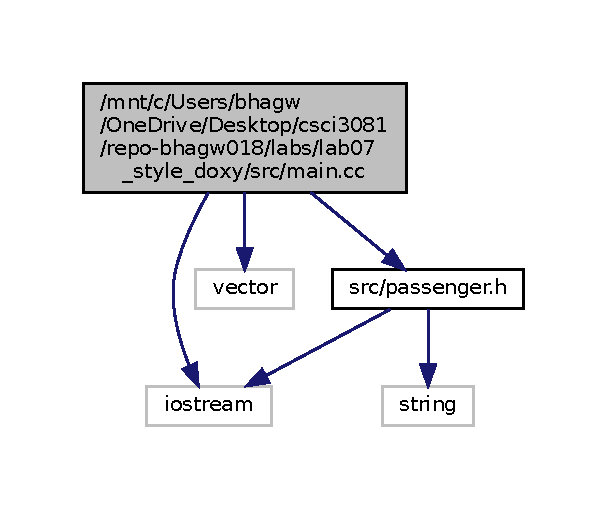
\includegraphics[width=292pt]{main_8cc__incl}
\end{center}
\end{figure}
\subsection*{Functions}
\begin{DoxyCompactItemize}
\item 
\mbox{\Hypertarget{main_8cc_ae66f6b31b5ad750f1fe042a706a4e3d4}\label{main_8cc_ae66f6b31b5ad750f1fe042a706a4e3d4}} 
int {\bfseries main} ()
\end{DoxyCompactItemize}
\subsection*{Variables}
\begin{DoxyCompactItemize}
\item 
\mbox{\Hypertarget{main_8cc_a9717e7bbecb906637e86cef6da3d83c2}\label{main_8cc_a9717e7bbecb906637e86cef6da3d83c2}} 
{\bfseries return}
\end{DoxyCompactItemize}


\subsection{Detailed Description}
\begin{DoxyCopyright}{Copyright}
2019 3081 Staff, All rights reserved. 
\end{DoxyCopyright}

\hypertarget{passenger__factory_8cc}{}\section{/mnt/c/\+Users/bhagw/\+One\+Drive/\+Desktop/csci3081/repo-\/bhagw018/labs/lab07\+\_\+style\+\_\+doxy/src/passenger\+\_\+factory.cc File Reference}
\label{passenger__factory_8cc}\index{/mnt/c/\+Users/bhagw/\+One\+Drive/\+Desktop/csci3081/repo-\/bhagw018/labs/lab07\+\_\+style\+\_\+doxy/src/passenger\+\_\+factory.\+cc@{/mnt/c/\+Users/bhagw/\+One\+Drive/\+Desktop/csci3081/repo-\/bhagw018/labs/lab07\+\_\+style\+\_\+doxy/src/passenger\+\_\+factory.\+cc}}
{\ttfamily \#include $<$random$>$}\newline
{\ttfamily \#include $<$string$>$}\newline
{\ttfamily \#include \char`\"{}src/passenger\+\_\+factory.\+h\char`\"{}}\newline
Include dependency graph for passenger\+\_\+factory.\+cc\+:\nopagebreak
\begin{figure}[H]
\begin{center}
\leavevmode
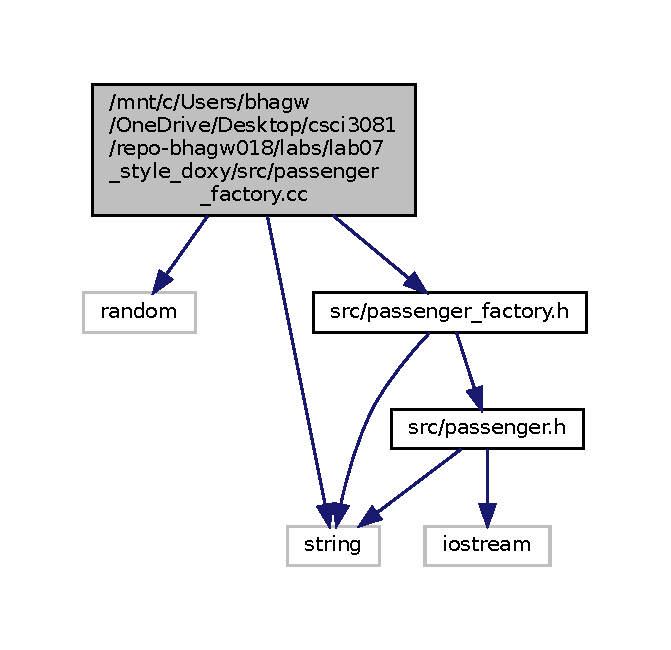
\includegraphics[width=322pt]{passenger__factory_8cc__incl}
\end{center}
\end{figure}
\subsection*{Functions}
\begin{DoxyCompactItemize}
\item 
\mbox{\Hypertarget{passenger__factory_8cc_af34adcff7354e7e8d172f7a97bc05d68}\label{passenger__factory_8cc_af34adcff7354e7e8d172f7a97bc05d68}} 
std\+::mt19937 {\bfseries e} (dev())
\item 
\mbox{\Hypertarget{passenger__factory_8cc_a1d818b31bbf5715a76ee321d8a0993e0}\label{passenger__factory_8cc_a1d818b31bbf5715a76ee321d8a0993e0}} 
std\+::uniform\+\_\+int\+\_\+distribution$<$ std\+::mt19937\+::result\+\_\+type $>$ {\bfseries dist} (1, 1000)
\end{DoxyCompactItemize}
\subsection*{Variables}
\begin{DoxyCompactItemize}
\item 
\mbox{\Hypertarget{passenger__factory_8cc_ad768868c172722a84c70801c1382438f}\label{passenger__factory_8cc_ad768868c172722a84c70801c1382438f}} 
std\+::random\+\_\+device {\bfseries dev}
\end{DoxyCompactItemize}


\subsection{Detailed Description}
\begin{DoxyCopyright}{Copyright}
2019 3081 Staff, All rights reserved. 
\end{DoxyCopyright}

\hypertarget{passenger__factory_8h}{}\section{/mnt/c/\+Users/bhagw/\+One\+Drive/\+Desktop/csci3081/repo-\/bhagw018/labs/lab07\+\_\+style\+\_\+doxy/src/passenger\+\_\+factory.h File Reference}
\label{passenger__factory_8h}\index{/mnt/c/\+Users/bhagw/\+One\+Drive/\+Desktop/csci3081/repo-\/bhagw018/labs/lab07\+\_\+style\+\_\+doxy/src/passenger\+\_\+factory.\+h@{/mnt/c/\+Users/bhagw/\+One\+Drive/\+Desktop/csci3081/repo-\/bhagw018/labs/lab07\+\_\+style\+\_\+doxy/src/passenger\+\_\+factory.\+h}}
{\ttfamily \#include $<$string$>$}\newline
{\ttfamily \#include \char`\"{}src/passenger.\+h\char`\"{}}\newline
Include dependency graph for passenger\+\_\+factory.\+h\+:\nopagebreak
\begin{figure}[H]
\begin{center}
\leavevmode
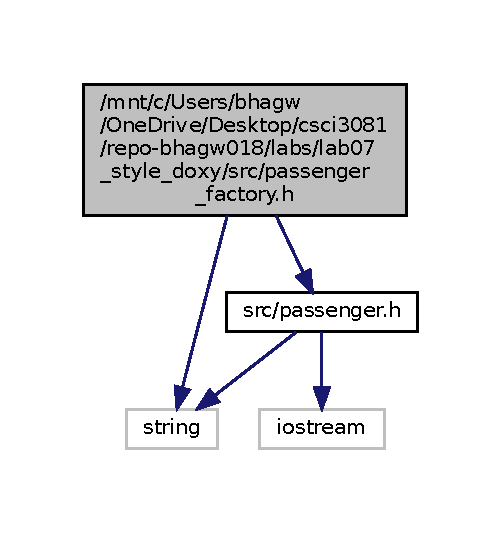
\includegraphics[width=241pt]{passenger__factory_8h__incl}
\end{center}
\end{figure}
This graph shows which files directly or indirectly include this file\+:\nopagebreak
\begin{figure}[H]
\begin{center}
\leavevmode
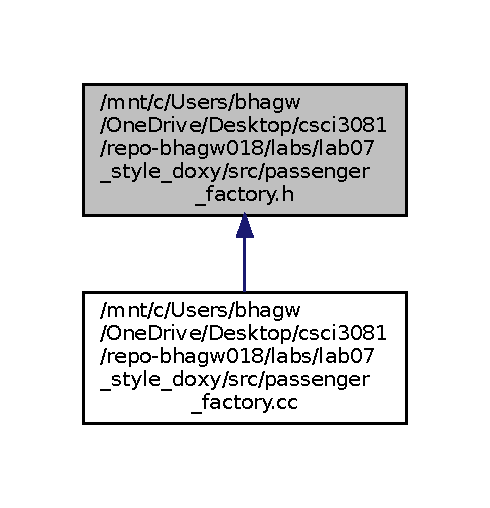
\includegraphics[width=235pt]{passenger__factory_8h__dep__incl}
\end{center}
\end{figure}
\subsection*{Classes}
\begin{DoxyCompactItemize}
\item 
class \hyperlink{classPassengerFactory}{Passenger\+Factory}
\begin{DoxyCompactList}\small\item\em The main class for the generation of passengers. \end{DoxyCompactList}\end{DoxyCompactItemize}


\subsection{Detailed Description}
\begin{DoxyCopyright}{Copyright}
2019 3081 Staff, All rights reserved. 
\end{DoxyCopyright}

%--- End generated contents ---

% Index
\backmatter
\newpage
\phantomsection
\clearemptydoublepage
\addcontentsline{toc}{chapter}{Index}
\printindex

\end{document}
